\section{Exercise nine}

Consider the following code: 
\begin{verbnobox}[\verbarg]
LD F1, 0(R1)
FADD F2, F2, F3
ADDI R3, R3, 8
LD F4, 0(R2)
FADD F5, F4, F2
FMULT F6, F1, F4
ADDI R5, R5, 1
LD R6, 0(R4)
SD F6, 0(R5)
SD F5, 0(R6)
\end{verbnobox}
We have: 
\begin{itemize}
    \item 3 RESERVATION STATIONS (RS1, RS2, RS3) + 3 LOAD/STORE unit (LDU1, LDU2, LDU3) with latency 3
    \item 3 RESERVATION STATIONS (RS4, RS5, RS6) + 3 FPUs (FPU1, FPU2, FPU3) with latency 3
    \item 2 RESERVATION STATIONS (RS7, RS8) + 1 Integer ALU ( ALU1) with latency 1
\end{itemize}
\begin{enumerate}
    \item Find all the conflicts. 
    \item Apply the Tomasulo algorithm. 
\end{enumerate}

\subsection*{Solution}
\begin{enumerate}
    \item The conflicts are the following: 
        \begin{itemize}
            \item RAW F0 I1-I6
            \item RAW F2 I2-I5
            \item RAW F4 I4-I5
            \item RAW F4 I4-I6
            \item RAW F6 I6-I9
            \item RAW F5 I5-I10
            \item RAW R5 I7-I9
            \item RAW R6 I8-I10
        \end{itemize}
    \item The final result of the Tomasulo algorithm is: 
        \begin{figure}[H]
            \centering
            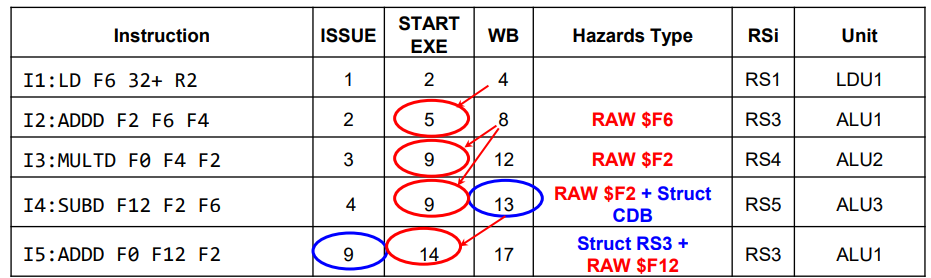
\includegraphics[width=1\linewidth]{images/tom.png}
        \end{figure}
\end{enumerate}